\section{L'atmospère}
	L'atmosphère terrestre est la mince couche de gaz qui entoure la Terre.
	
	On considère que l'atmosphère à une épaisseur d'environ 120 km, hauteur à laquelle le ralentissement lié à l'atmosphère devient notable.
	\subsection{Composition}
	
	L'atmosphère est composée d'un ensemble de gaz dont la proportion est constante pratiquement dans toutes l'atmosphère. Cet ensemble de gaz est appelé \textbf{air}. Un autre gaz, la vapeur d'eau, est souvent mélangé à cet air, en proportion variable selon le temps, le lieu et l'altitude. La proportion de vapeur d'eau que peut contenir l'air va jusqu'à environ 5~\%.
	
	L'air sec est composé de :
	\begin{table}[H]
	\centering
	\begin{tabular}{|l|c|}
		\hline
		Gaz & Proportion \\
		\hline
		\hline
		Azote ($N$) & 78~\% \\
		\hline
		Oxygène ($O$) & 21~\% \\
		\hline
		Argon ($Ar$) & 0,9~\% \\
		\hline
		Autres gaz (dont Dioxyde de carbone ($CO_2$)) & 0,1~\% \\
		\hline
	\end{tabular}
	\caption{Composition de l'atmosphère terrestre}
	\end{table}
	
	
	\subsection{Structure}
	L'atmosphère a été découpée en plusieurs couches successives, dont les limites ont été fixées sur la base des discontinuités des variations de température que l'on y rencontre.
	
	\begin{figure}[H]
			\centering
			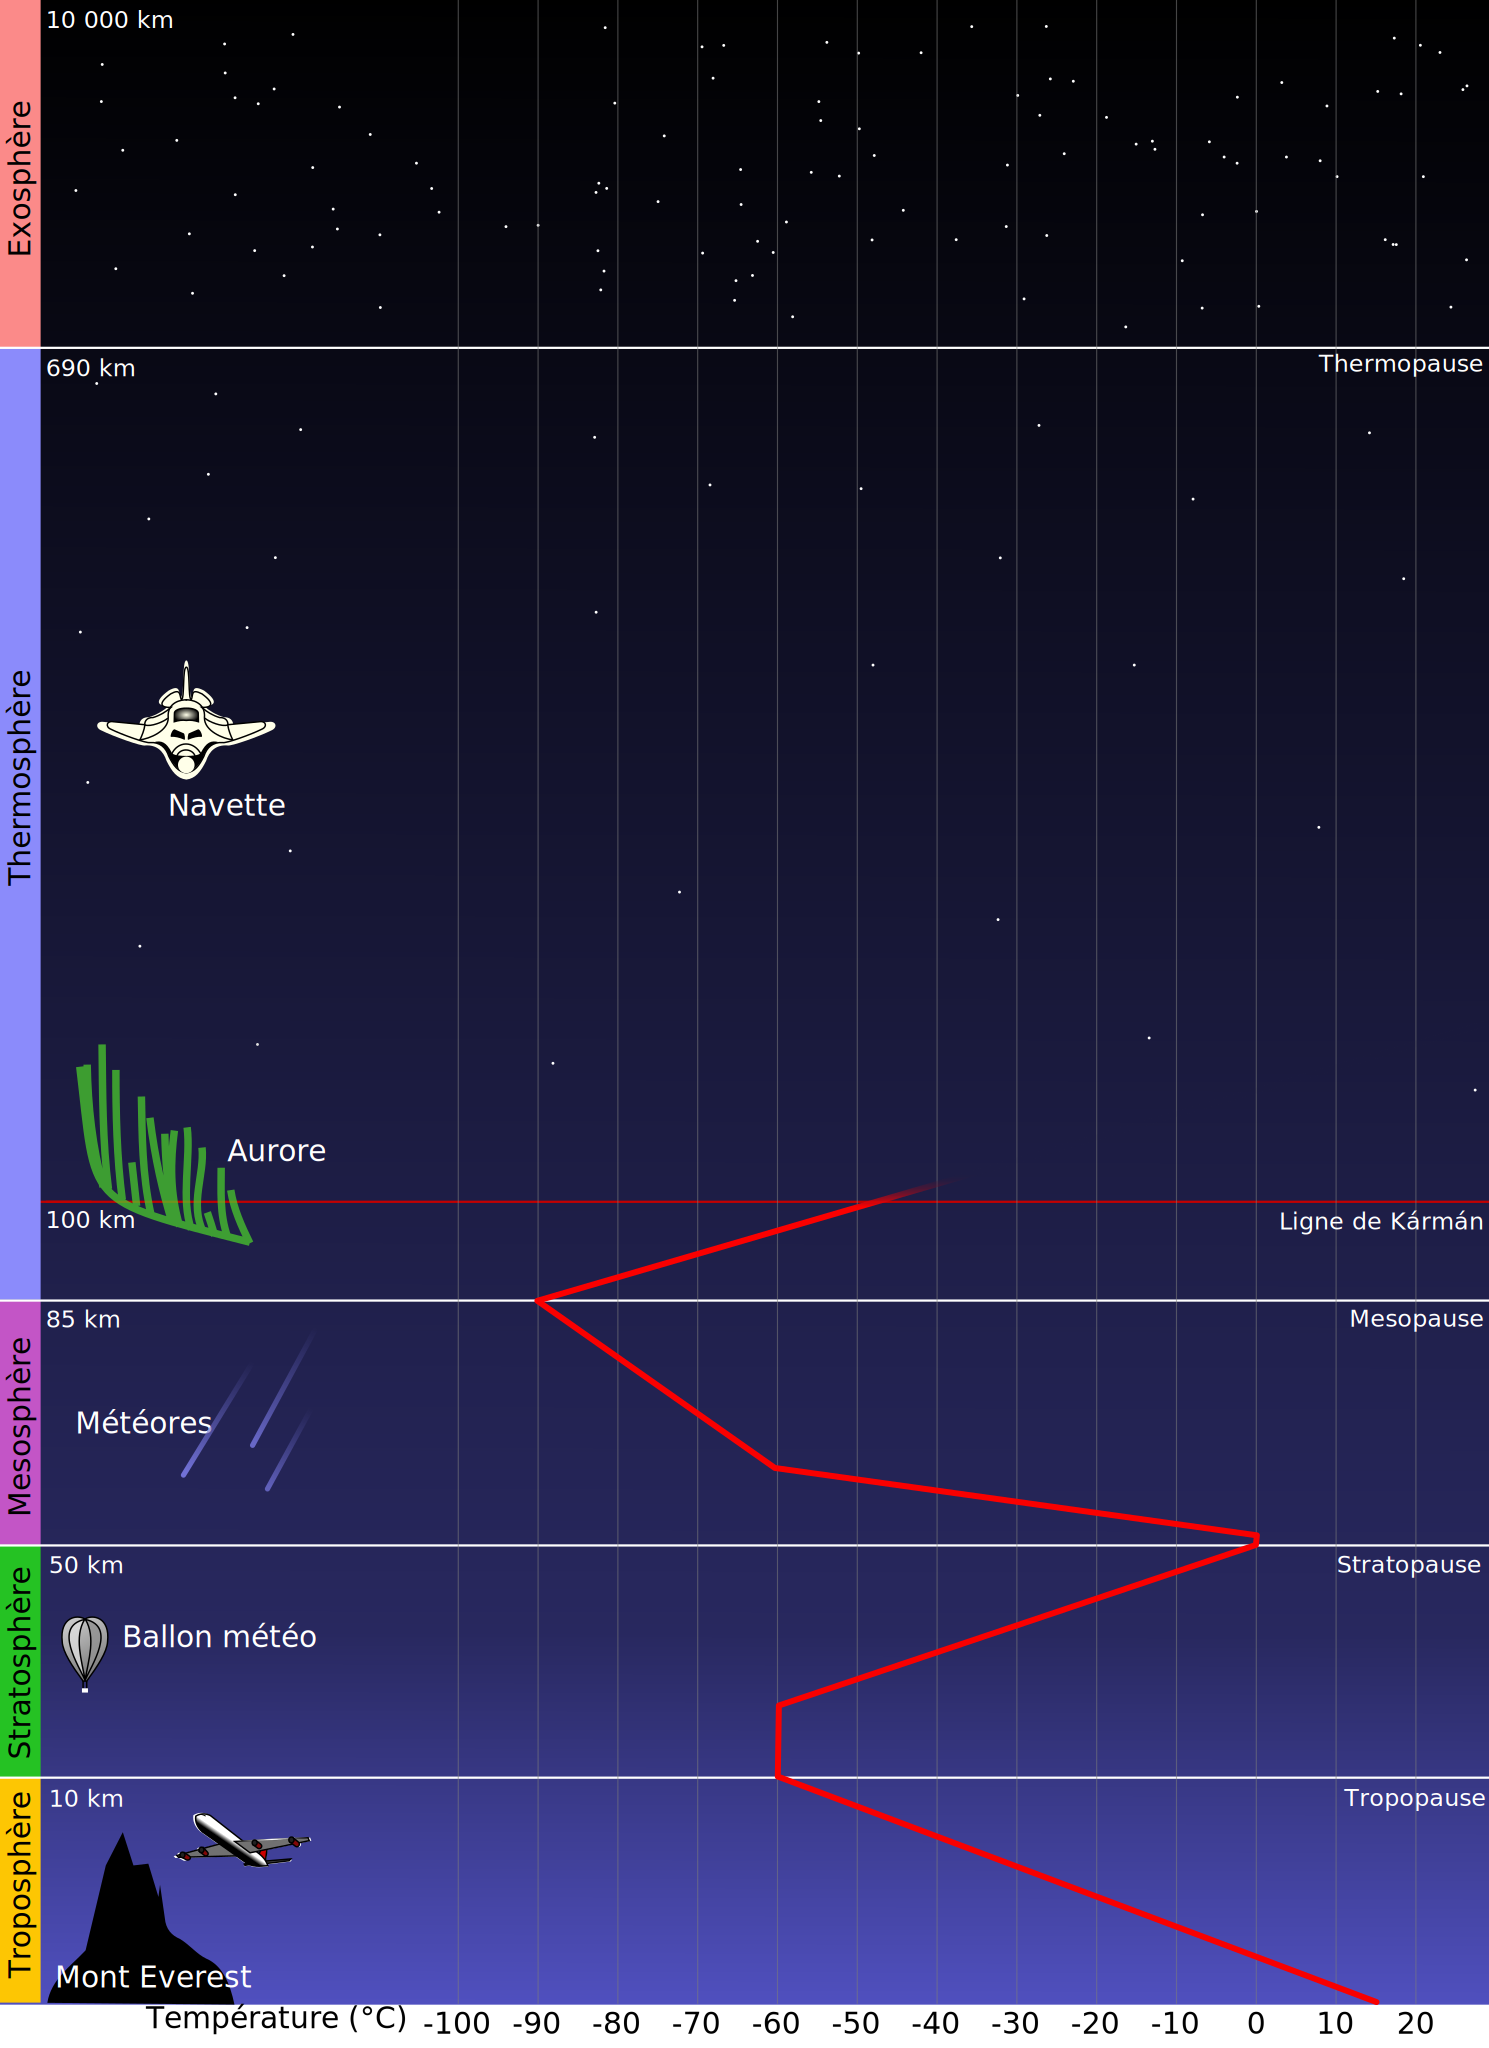
\includegraphics[width=0.8\linewidth]{03-Meteo/img/couchesAtmosphereTemperature.pdf}
			\legende{Schéma des couches de l'atmosphère, avec la courbe de température normale et le nom des limites}{img:couchesAtmosphereTemperature}
			\end{figure}	
			
	\subsection{La pression atmosphérique}
	La colonne d'air qui se trouve au dessus de nos têtes subit la gravité terrestre. Par conséquence, elle représente un poids, appelé pression atmosphérique.
	
	Cette pression peut-être mise en évidence grâce à des baromètres, des dispositifs prévus pour mesurer la valeur de cette pression.
	
	Cette pression a été mise en évidence par le physicien italien Evangelista Torricelli au début du \siecle{17}. Le physicien rempli un tube en verre fermé d'un côté avec du mercure, puis le retourne dans une cuve elle aussi remplie de mercure. Dans le tube, le mercure descend et se stabilise à une hauteur de 760 mm.
	
	\begin{figure}[H]
	\centering
	\begin{tikzpicture}[scale=1.7, every node/.style={scale=1.7}]
	\barometreTorricelli{760} 
	\draw [line width=0.5mm, -{Stealth[length=10mm, open, round]}]
          (-1,2) -- (-1,0.7);
    \draw [line width=0.5mm, -{Stealth[length=10mm, open, round]}]
          (1,2) -- (1,0.7);
	\end{tikzpicture}
	\legende{Baromètre de Torricelli au mercure, au niveau de la mer}{img:barometreTorricelli}
	\end{figure}
	
	La pression atmosphérique appuie en réalité sur le mercure contenu dans la cuve.
	
	\subsubsection{Variation de la pression atmosphérique avec l'altitude}
	Lorsque l'on se déplace verticalement dans l'atmosphère, la colonne d'air qui se trouve au dessus est moins haute. Par conséquence, la pression atmosphérique diminue lorsque l'on s'élève dans l'atmosphère.
	
	\begin{figure}[H]
		\ifdefined\activeranimations 
		\newcommand{\nbFramesAltitude}{101}
		\else
		\newcommand{\nbFramesAltitude}{1}
		\fi
		
		%760 mmHg à 0 m
		%200 mmHg à 10 000 m
		%=> 560 mmHg entre les 2, soit, pour 100 frames, 5.6
		%\newcommand{\altToMmHg}{((760-200)/\nbFramesAltitude)}
		%\newcommand{\altToMmHg}{0.2}
		
		\centering
		\begin{animateinline}[controls,loop]{8}
		    \multiframe{\nbFramesAltitude}{i=0+1}{
			\begin{tikzpicture}[x=1cm,y=1cm, scale=0.5, every node/.style={scale=0.5}]
				\echelleAltitudeMetres{10}{\i/10}
			\end{tikzpicture}
			\begin{tikzpicture}[scale=1.1, every node/.style={scale=1.1}]
				%\FPeval{\asoustraire}{clip(\i*\altToMmHg)}
				\FPeval{\result}{round((760-\i*5.6),0)}
				\barometreTorricelli{\result}		
			\end{tikzpicture}
			}
		\end{animateinline}
	\end{figure}